\documentclass[tikz,border=7pt]{standalone}
\usetikzlibrary{matrix,fit,positioning, arrows.meta, decorations.pathreplacing} 
\begin{document}
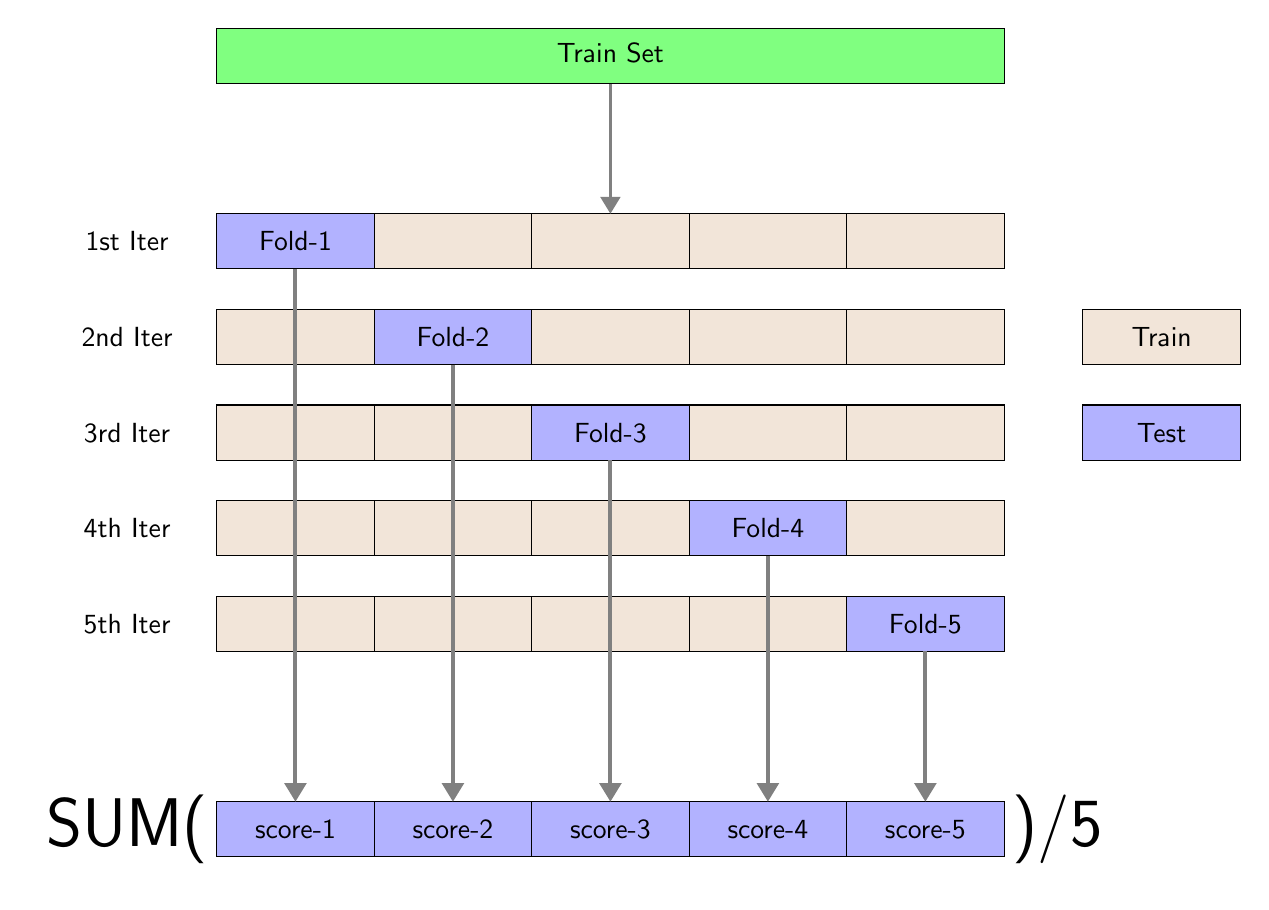
\begin{tikzpicture}[font=\sffamily,
%   Fold/.style={/utils/exec=\stepcounter{Fold}
% \pgfmathtruncatemacro{\itest}{ifthenelse(mod(\number\value{Fold},5)==int(1+\number\value{Fold}/5)
% || \number\value{Fold}==25,1,0)}
% \pgfmathsetmacro{\mycol}{{\LstCol}[\itest]},fill=\mycol,draw,
% node contents={Fold \pgfmathparse{int(mod(\number\value{Fold}-1,5)+1)}\pgfmathresult}
% },
  standard/.style={inner sep=0pt,align=center,draw,%text
    % height=1.25em,
    minimum height = 7mm,
    text depth=0.5em},
  decoration={brace},
  oneblock/.style={transform shape,minimum width=1cm,draw}]
    \matrix (M) [
        matrix of nodes,
        nodes={
%          text height=1.25em,
%          text depth=2cm,
            minimum height = 7mm,
            minimum width = 2cm,
           outer sep=0,
           anchor=center,
           draw,fill=brown!20 % <-added
        },
        column 1/.style={
            nodes={draw=none,fill=none}, % <-- added fill=none
            minimum width = 4cm
          },
        column 7/.style={
            nodes={draw=none,fill=none,align=left}, % <-- added fill=none
            minimum width = 4cm
        },
        row sep=5mm, column sep=-\pgflinewidth,
        nodes in empty cells,
        e/.style={fill=blue!30},
        alignleft/.style={draw=none, fill=none,align=left}
      ]
      {
        1st Iter & |[e]| Fold-1& & & & &|[draw=none, fill=none]|\\
        2nd Iter & & |[e]| Fold-2& & & &|[draw=none, fill=none]| \\
        3rd Iter & & & |[e]| Fold-3& & &|[draw=none, fill=none]| \\
        4th Iter & & & & |[e]| Fold-4& &|[draw=none, fill=none]| \\        
        5th Iter & & & & & |[e]| Fold-5 &|[draw=none, fill=none]|\\
        |[draw=none,fill=none]| &|[draw=none, fill=none]|
        &|[draw=none, fill=none]| & |[draw=none,
        fill=none]|&|[draw=none, fill=none]| &|[draw=none, fill=none]| &|[draw=none, fill=none]|\\
        {\Huge SUM(} & |[e]|score-1& |[e]|score-2& |[e]|score-3&
        |[e]|score-4&|[e]|score-5 & {\Huge )/5\hspace*{1cm}}\\
      };
      % \draw (M-1-3.north west) ++(0,2mm) coordinate (LT) edge[|<->|, >= latex] node[above]{Train} (LT-|M-1-6.north east); % changed 5 to 7
      %  \draw (M-1-2.north west) ++(0,2mm) coordinate (LT) edge[|<->|,
      %  >= latex] node[above]{Test} (LT-|M-1-2.north east);
       % geschweifte Klammer auf rechter Seite
%       \draw[thick,decorate] ([yshift=-3pt]M.north east) -- ([yshift=3pt]M.south east)
%       node[midway,right]{Finding parameters};
       % big bars above matrix
       \node[fit=(M-1-2) (M-1-6), fill=green!50,
       yshift=2cm, standard, anchor=south](trs) {Train Set};
       \draw[->][black!50, line
           width=1.2pt,-Triangle](trs) -- (M-1-4);
       \node[oneblock, minimum height = 7mm, minimum width = 2cm,
       anchor=west,right=of M-2-6,fill=brown!20,outer sep=0mm] (A1)
       {Train};
       \node[oneblock, minimum height = 7mm, minimum width = 2cm,
       anchor=east,right=of M-3-6,fill=blue!30,outer sep=0mm] (A2) {Test};       
      % dots
      %\node [below=3pt] at (M-3-5.south east) {$\cdots$};

      % fold labels and arrows
       \foreach [
             count=\row,
             evaluate={\col=ifthenelse(\row==99, % if fourth row
                                       int(\row+3), % use seventh column
                                       int(\row+1)) % else use column row+1
                       }
                ] \txt in {1,2,3,4,5}
         {
           % \node [below] at (M-\row-\col.south) {Fold-\txt};
           \draw[->][black!50, line
           width=0.5mm,-Triangle](M-\row-\col.south) -- (M-7-\col.north);
           % \draw [black!30,line width=1mm,-Triangle] (M-\row-6.east) ++(2mm,0) -- ++(7mm,0) node[black, right] {$E_{\txt}$}; 
          }

  \end{tikzpicture}
\end{document}
%%% Local Variables:
%%% mode: latex
%%% TeX-master: t
%%% End:
